\documentclass{standalone}

\usepackage{tkz-fct}
\usepackage{tkz-euclide}
\usepackage{color}
\renewcommand*\familydefault{\sfdefault}
\usepackage{sansmath}
\sansmath
\definecolor{gray75}{gray}{0.75}
\begin{document}
 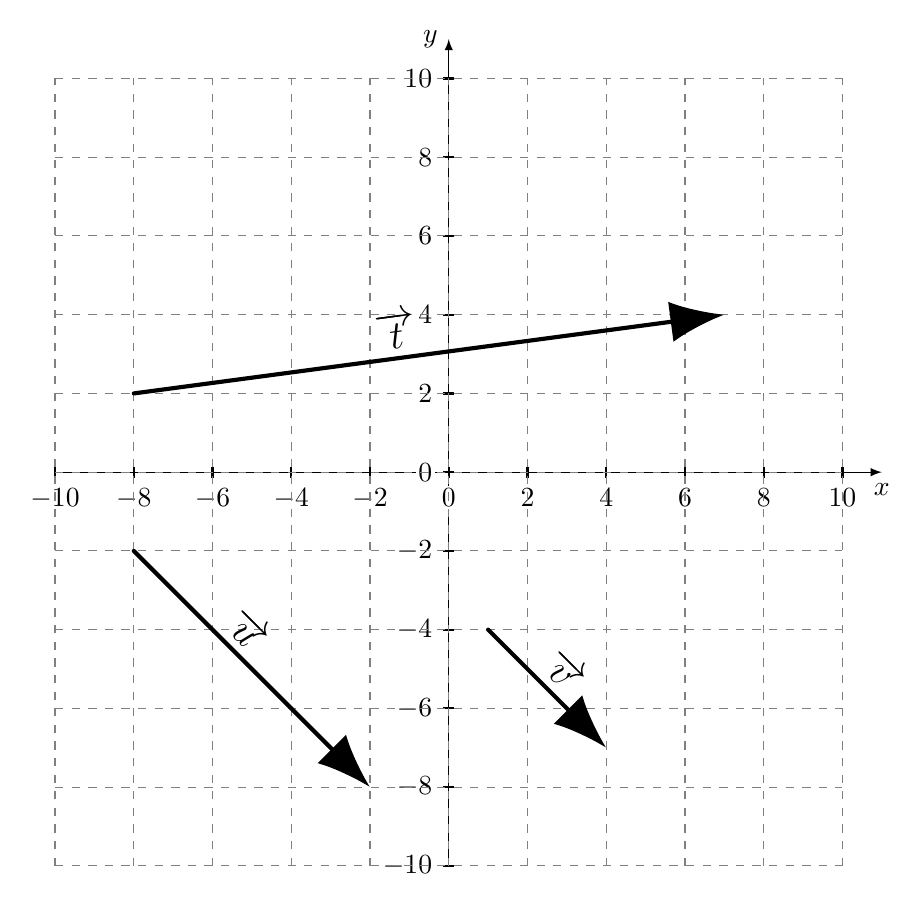
\begin{tikzpicture}
   \tkzInit[xmax=10,ymax=10,xmin=-10,ymin=-10, ystep=2, xstep=2]
   \tkzDrawX
   \tkzDrawY
   \tkzLabelX
   \tkzLabelY
   \begin{scope}[dashed]
     \tkzGrid
   \end{scope}
   \tikzset{vector style/.style={>={Latex[scale=2]},->}}
   \tkzDefPoints{-8/2/A, 7/4/B, 1/-4/C, 4/-7/D,-8/-2/E, -2/-8/F}
   \tkzDrawSegment[line width=1.5pt,vector style](C,D)
   \tkzDrawSegment[line width=1.5pt,vector style](A,B)
   \tkzLabelSegment[above, sloped](C,D){\Large $\overrightarrow{v}$}
   \tkzLabelSegment[above left, sloped](A,B){\Large $\overrightarrow{t}$}
   \tkzLabelSegment[above left, sloped](E,F){\Large $\overrightarrow{u}$}
   \tkzDrawSegment[line width=1.5pt,vector style](E,F)

\end{tikzpicture}
\end{document}
